\documentclass[a4papar,landscape]{article}

\usepackage{multicol}
\columnsep=10pt
\columnseprule=1pt

\usepackage{amsmath}

\usepackage{graphicx}
\usepackage{xcolor}
\usepackage{xeCJK}
\setCJKmainfont{WenQuanYi Zen Hei}
\setmonofont{DejaVu Sans Mono}
\setsansfont{DejaVu Sans Mono}
\usepackage[colorlinks=true,linkcolor=black]{hyperref}


\usepackage{setspace}
\topmargin=-0.5in
\evensidemargin=-0.25in
\oddsidemargin=-0.25in
\textwidth=10.0in
\textheight=7.0in
\headsep=0.25in
\usepackage{titlesec}
\titlespacing{\section}{0pt}{3pt}{0pt}
\titlespacing{\subsection}{0pt}{1pt}{0pt}
\titlespacing{\subsubsection}{0pt}{1pt}{0pt}

\usepackage{fancyhdr}
\pagestyle{myheadings}
\markright{Tsinghua U}

\usepackage{listings}
\lstset{
	language=C++,
	basicstyle=\ttfamily \footnotesize,
	numberstyle=\it\scriptsize\sffamily,
	keywordstyle=\bfseries,
	identifierstyle=,
	commentstyle=\color{gray},
	stringstyle=,
	showstringspaces=false,
%	frame=single,
	tabsize=4,
%	numbers=left,
%	numbersep=2pt,
}

\begin{document}
%%%%%%%%%%%%%%%%%%%%%%%%%%%%%%%%%%%%%%%%%%%%%%%%%%%%%%%
%%%%%%%%%%%%%%%%%%%%%%%%%%%%%%%%%%%%%%%%%%%%%%%%%%%%%%%
%\begin{titlepage}
%\begin{center}
	%\textsc{} \\[2.0cm]
	 
	%\textsc{\LARGE Tsinghua Univertisy} \\[1.0cm]

	%\textsc{\huge  ACM/ICPC World Final 2014 Reference} \\[2.5cm]

	%{\Huge \bfseries NowOrNever} \\[2cm]

	%\Large
	%\begin{minipage}{0.4\textwidth}
	%\begin{flushleft}
		%\emph{Coach:}\\
		%Xiaojun \textsc{Wu}
		%\newline
		%\newline
	%\end{flushleft}
	%\end{minipage}	
	%\begin{minipage}{0.4\textwidth}
	%\begin{flushright}
		%\emph{Gamers:} \\
		%Qinshi \textsc{Wang} \\
		%Lijie \textsc{Chen} \\
		%Qiwei \textsc{Feng} \\
	%\end{flushright}
	%\end{minipage}

	%\vfill

	%{\large \today}
%\end{center}
%\end{titlepage}


\begin{multicols}{2}
\setcounter{tocdepth}{5}
\tableofcontents
\newpage
%%%%%%%%%%%%%%%%%%%%%%%%%%%%%%%%%%%%%%%%%%%%%%%%%%%%%%%
%%%%%%%%%%%%%%%%%%%%%%%%%%%%%%%%%%%%%%%%%%%%%%%%%%%%%%%

\section{计算几何}

	\subsection{2D-圆}
		\lstinputlisting{codes/geo/2d-circle.h}
	\subsection{2D-多边形与凸包}
		\lstinputlisting{codes/geo/2d-polygon.h}
	\subsection{3D-基础操作}
		\lstinputlisting{codes/geo/3d-basic.h}
	\subsection{3D-旋转}
		\lstinputlisting{codes/geo/3d-rotate.h}
	\subsection{3D-$O(n^2)$凸包}
		\lstinputlisting{codes/geo/3d-convex.h}
	\lstset{language=Java}
	\subsection{Delaunay}
		\lstinputlisting{codes/geo/delaunay.java}
	\lstset{language=C++}
	\subsection{平面图}
		\lstinputlisting{codes/geo/planar-graph.cpp}

\section{数据结构}

	\subsection{动态树}
		\lstinputlisting{codes/ds/dynamic-tree.h}

\section{图论}

	\subsection{任意图匹配(带花树)}
		\lstinputlisting{codes/graph/blossom.cpp}
	\subsection{Dinic}
		\lstinputlisting{codes/graph/dinic.h}
	\subsection{Hopcroft}
		\lstinputlisting{codes/graph/hopcroft.h}
	\subsection{SAP}
		\lstinputlisting{codes/graph/sap.cpp}
	\subsection{Directed MST}
		\lstinputlisting{codes/graph/directed-mst.cpp}
	\subsection{无向图最小割}
		\lstinputlisting{codes/graph/n-mincut.h}
	\subsection{点分治}
		\lstinputlisting{codes/graph/point-divide.cpp}
	\lstset{language=Java}
	\subsection{2-SAT}
		\lstinputlisting{codes/graph/TWOSAT.java}
	\lstset{language=C++}

\section{数学}

	\subsection{行列式计算}
		\lstinputlisting{codes/math/det.h}
	\subsection{质数测试(OLD!!)}
		\lstinputlisting{codes/math/factors.h}
	\subsection{高精度乘法(Karatsuba)}
		\lstinputlisting{codes/math/multiply-kara.h}
	\subsection{高精度乘法(FFT)}
		\lstinputlisting{codes/math/multiply-fft.h}
	\subsection{快速矩阵乘法(Strassen) [abstract]}
		\lstinputlisting{codes/math/mat-mul.txt}
	\subsection{直线下有多少格点}
		求$\sum_{k=0}^{n-1} \lceil \frac{a+bk}{m}\rceil$,
			$a,b>0$.
		\lstinputlisting{codes/math/grids.h}

		%Want
		%\begin{equation*}
			%\begin{pmatrix} C_1 & C_2 \\ C_3 & C_4 \end{pmatrix}
			%=
			%\begin{pmatrix} A_1 & A_2 \\ A_3 & A_4 \end{pmatrix}
			%\begin{pmatrix} B_1 & B_2 \\ B_3 & B_4 \end{pmatrix}.
		%\end{equation*}
		%Let
		%\begin{equation*} \begin{split}
			%M_1 &= ( \\
			%M_2 &= b \\
		%\end{split} \end{equation*}


\section{其他}

	\subsection{后缀自动机}
		\lstinputlisting{codes/others/sam.cpp}

	\subsection{Dancing Links}
		\lstinputlisting{codes/others/dlx.h}
	\subsection{字符串的最小表示}
		\lstinputlisting{codes/others/min-rep.h}

	\lstset{language=Java}
	\subsection{JAVA Input}
		\lstinputlisting{codes/others/read.java}
	\lstset{language=C++}
	
\section{Additional Section}
	(Additional Section.)\\
	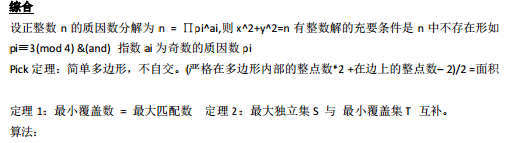
\includegraphics[width=\linewidth]{codes/addi/math1.png}
	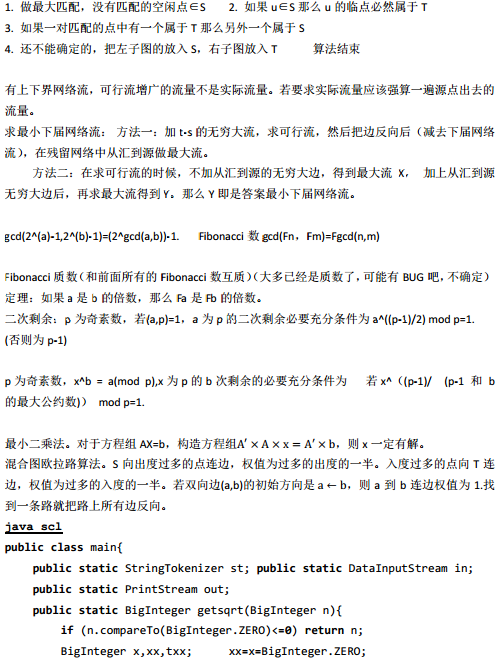
\includegraphics[width=\linewidth]{codes/addi/math2.png}
	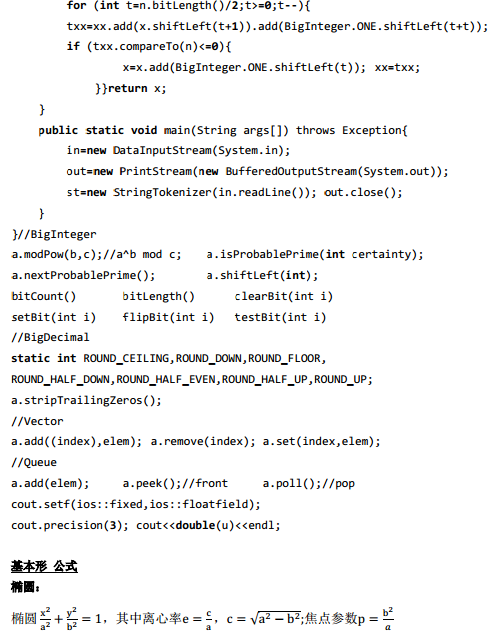
\includegraphics[width=\linewidth]{codes/addi/math3.png}
	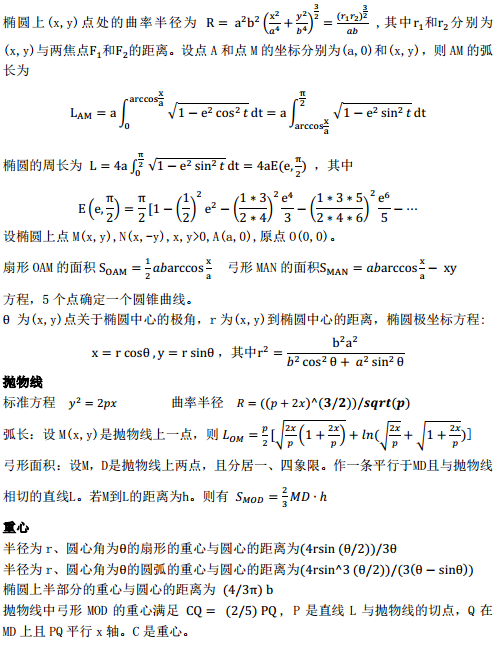
\includegraphics[width=\linewidth]{codes/addi/math4.png}
	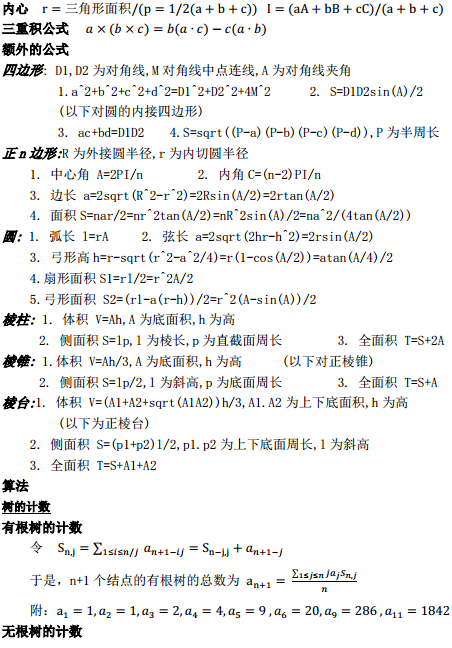
\includegraphics[width=\linewidth]{codes/addi/math5.png}
	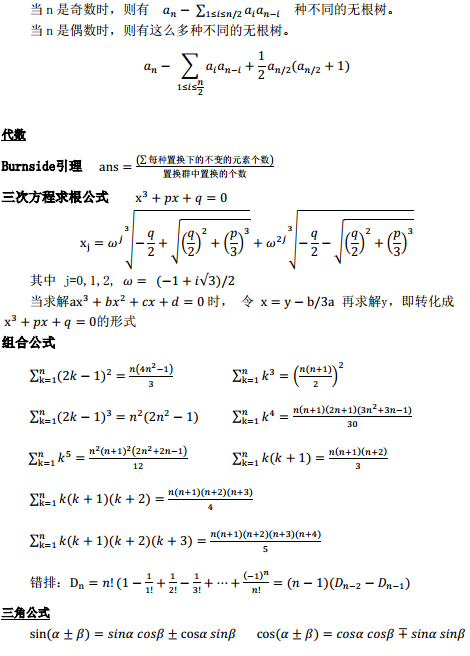
\includegraphics[width=\linewidth]{codes/addi/math6.png}
	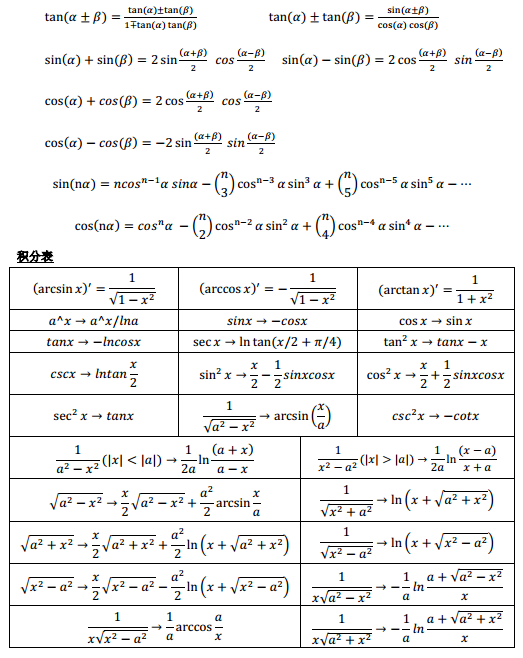
\includegraphics[width=\linewidth]{codes/addi/math7.png}
	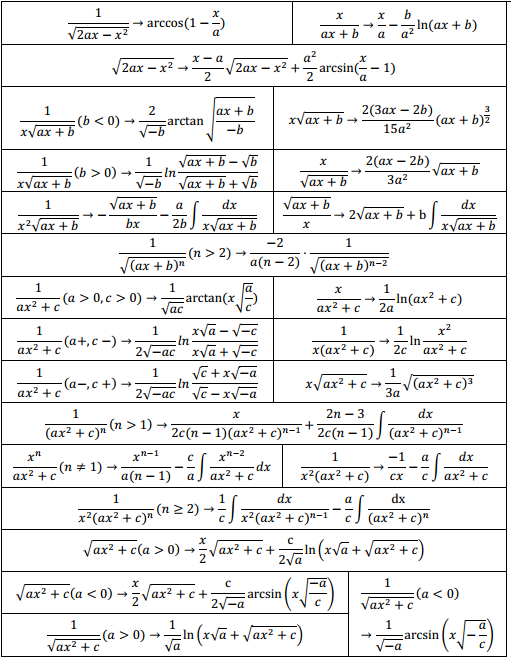
\includegraphics[width=\linewidth]{codes/addi/math8.png}
	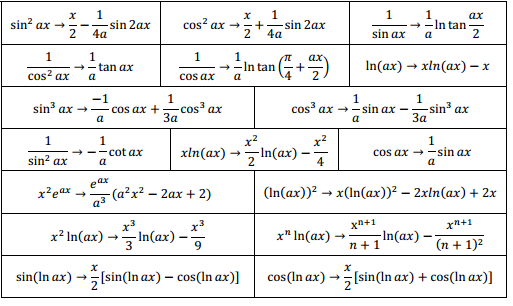
\includegraphics[width=\linewidth]{codes/addi/math9.png}


%%%%%%%%%%%%%%%%%%%%%%%%%%%%%%%%%%%%%%%%%%%%%%%%%%%%%%%
%%%%%%%%%%%%%%%%%%%%%%%%%%%%%%%%%%%%%%%%%%%%%%%%%%%%%%%
\end{multicols}
\end{document}
